\documentclass[10pt]{report}

\usepackage[
  scale=0.875,
  stdmathitalics=true,
  stdmathdigits=true]{lucimatx}
\linespread{1.02}
%\usepackage{helvet}

\usepackage{fancyvrb}
\usepackage{amsmath}
% \usepackage{amssymb}
\usepackage{graphicx}
\usepackage[usenames,dvipsnames,svgnames,table]{xcolor}


\setlength{\paperheight}{3in}
\setlength{\paperwidth}{4in}
\pdfpagewidth=\paperwidth
\pdfpageheight=\paperheight

\setlength{\textwidth}{3.75in}
\setlength{\textheight}{2.5in}

\setlength{\oddsidemargin}{-1.0in}
\setlength{\evensidemargin}{-1.0in}
\setlength{\topmargin}{-1.25in}

\newcommand{\sld}[1]{\newpage{\noindent\LARGE \ \ \
    \textcolor{MidnightBlue}{\bfseries #1}}\vspace*{4pt}}

\newcommand{\code}[1]{{\tt #1}}
\newcommand{\spc}{\hspace*{0.25in}}

\newcounter{gmlrx}
\newcounter{gmlry}
\newcommand{\gmnode}[3]{\put(#1,#2){\circle{20}}\put(#1,#2){\makebox(0,0){$#3$}}}
\newcommand{\gmplate}[5]{
\setcounter{gmlrx}{#1}\addtocounter{gmlrx}{#3}
\setcounter{gmlry}{#2}\addtocounter{gmlry}{-#4}
\put(#1,#2){\line(1,0){#3}}
\put(#1,#2){\line(0,-1){#4}}
\put(\value{gmlrx},\value{gmlry}){\line(-1,0){#3}}
\put(\value{gmlrx},\value{gmlry}){\line(0,1){#4}}
\setcounter{gmlrx}{#1}\addtocounter{gmlrx}{5}
\setcounter{gmlry}{#2}\addtocounter{gmlry}{-6}
\put(\value{gmlrx},\value{gmlry}){\makebox(0,0){$#5$}}
}

\newcommand{\myemph}[1]{{\color{MidnightBlue}{\bfseries #1}}}
\newcommand{\mypart}[2]{{\newpage 
\mbox{ }
\vfill
\noindent\spc\color{MidnightBlue}{\LARGE\bfseries #1\\[10pt]\spc\Huge{#2}}
\vfill\vfill}
\mbox{ }}

\begin{document}
\sf%
\vspace*{6pt}
%
\noindent
\spc{\huge\bfseries \color{MidnightBlue}{Stan}}
\\[8pt]
\spc{\Large\bfseries \color{MidnightBlue}{Probabilistic Programming Language}}
\\
\vfill
\noindent
\spc\spc{\slshape\footnotesize Core Development Team:}
\\[2pt]
\spc\spc{\small Andrew Gelman, \  \myemph{Bob Carpenter}, \  Matt Hoffman}
\\
\spc\spc{\small Daniel Lee, \  Ben Goodrich, \  Michael Betancourt, \ }
\\
\spc\spc{\small Marcus Brubaker, \   Jiqiang Guo, \  Peter Li, \ }
\\
\spc\spc{\small Allen Riddell, \  Marco Inacio}
\vfill
\mbox{ } 
\hfill

\includegraphics[width=27.5pt]{img/stanlogo-main.pdf}\hspace*{9pt}
\\
\spc{\footnotesize Paris-Dauphine 2014}
\hfill 
{\footnotesize \tt mc-stan.org}

\sld{What is Stan?}

\begin{itemize}
\item Stan is an \myemph{imperative} probabilistic programming language
\vspace*{-12pt}
\begin{itemize}\footnotesize
\item  cf., BUGS: declarative; \ Church: functional; \ Figaro: object-oriented
\end{itemize}
\item Stan \myemph{program}
\vspace*{-4pt}
\begin{itemize}\small
\item declares variables
\item codes log posterior (penalized likelihood)
\end{itemize}
\item Stan \myemph{inference}
\vspace*{-4pt}
\begin{itemize}\small
\item MCMC for full Bayesian inference
\item MLE for point estimation
\end{itemize}
\item Stan is \myemph{open source} \ {\footnotesize (BSD core C++, GPLv3 interfaces)}
\\
{\footnotesize hosted on GitHub; uses Eigen matrix lib, Boost, googletest
  C++ lib}
\end{itemize}

\sld{Who's Using Stan?}
\begin{itemize}
\item 750+ registrations for mailing list across the physical,
biomedical, and social sciences, plus engineering, finance and marketing

\item Subjects of Papers on Google Scholar in the sciences
\\
{\footnotesize clinical drug
trials, general computational statistics, entomology, opthalmology,
neurology, sociology and population dynamics, genomics, agriculture,
psycholinguistics, molecular biology, population dynamics, materials
engineering, botany, astrophysics, oceanography, election prediction,
fisheries, cancer biology, public health and epidemiology, population
ecology, collaborative filtering for recommender systems, climatology,
educational testing, natural language processing}
\end{itemize}

\sld{Books and Model Sets}
%
\begin{itemize}
\item 400+ page core language tutorial manual
\item separate installation, getting started, interface manuals 
\\ {\footnotesize  RStan, PyStan, CmdStan}
\item BUGS and JAGS examples (all 3 volumes), 
\item Gelman and Hill, {\slshape Data Analysis Using Regression and
    Multilevel/Hierarchical Models}
\item Wagenmakers and Lee, {\slshape Bayesian Cognitive Modeling}
\item two other books in progress
\end{itemize}

\mypart{Part I}{Stan Front End}

\sld{Interface Languages}

\begin{itemize}
\item \myemph{Platforms}
\\
Linux, Mac OS X, Windows
\item \myemph{C++ API}
\\
{\footnotesize portable, standards compliant (C++03 now, moving to C++11)}
\item \myemph{Interfaces}
\vspace*{-4pt}
\begin{itemize}\footnotesize
\item \myemph{CmdStan}: Command-line or shell interface (direct executable)
\item \myemph{RStan}: R interface (Rcpp in memory)
\item \myemph{PyStan}: Python interface (Cython in memory)
\item \myemph{MStan$^*$}: MATLAB interface (lightweight external process)
\item \myemph{JuliaStan$^*$}: Julia interface (lightweight external process)
\end{itemize}
{\footnotesize ${}^*$ User contributed}
\end{itemize}
\vfill

\sld{Example: \ Bernoulli}
\vfill
\spc\spc
\begin{minipage}[t]{0.8\textwidth}
\begin{Verbatim}
data {
  int<lower=0> N;
  int<lower=0,upper=1> y[N];
}
parameters {
  real<lower=0,upper=1> theta;
} 
model {
  y ~ bernoulli(theta);
}
\end{Verbatim}
\end{minipage}
\vfill
\vfill
\vfill
\mbox{ } \hfill {\small\slshape notes: {\tt theta} uniform on $[0,1]$, \ {\tt y} vectorized}
\vfill


\sld{RStan Execution}

\begin{minipage}[t]{\textwidth}
\footnotesize
\begin{Verbatim}
> N <- 5;   y <- c(0,1,1,0,0);
> fit <- stan("bernoulli.stan", data = c("N", "y"));
> print(fit, digits=2)
\end{Verbatim}
\vspace*{1pt}
\begin{Verbatim}[fontshape=sl]
Inference for Stan model: bernoulli.
4 chains, each with iter=2000; warmup=1000; thin=1; 

       mean  se_mean    sd   2.5%    50%  97.5%  n_eff  Rhat
theta  0.43     0.01  0.18   0.11   0.42   0.78   1229     1
lp__  -5.33     0.02  0.80  -7.46  -5.04  -4.78   1201     1
\end{Verbatim}
\vspace*{6pt}
\begin{Verbatim}
> hist( extract(fit)$theta )
\end{Verbatim}
\vspace*{-24pt}
\hfill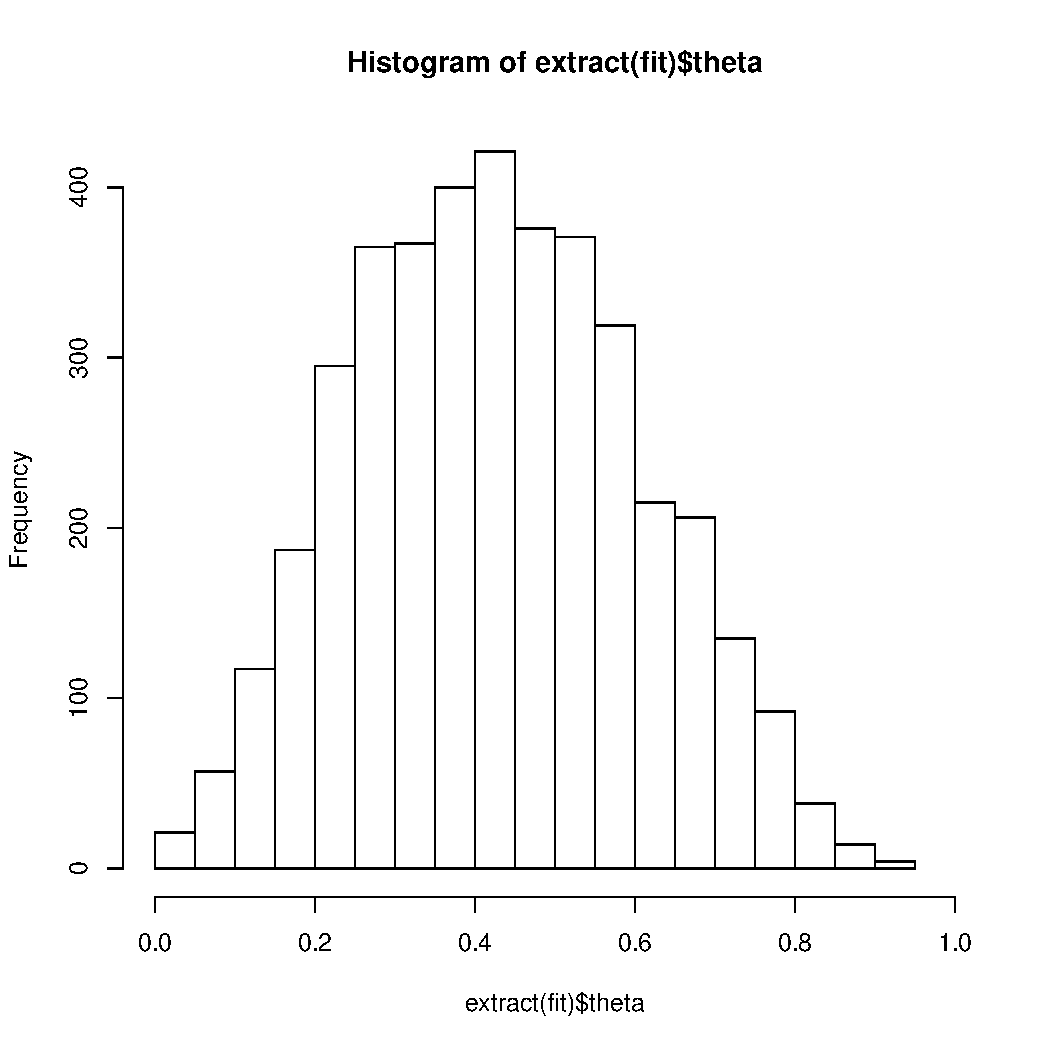
\includegraphics[width=1.25in,height=0.9in]{img/bernoulli-posterior-histo.pdf}
\hspace*{24pt}
\end{minipage}

\sld{Basic Program Blocks}

\begin{itemize}
\item \myemph{\tt\bfseries data} \ (once) 
\vspace*{-4pt}
\begin{itemize}\small
\item {\slshape content}: declare data types, sizes, and constraints
\item {\slshape execute}: read from data source, validate constraints
\end{itemize}
%
\item \myemph{\tt\bfseries parameters} \ (every log prob eval)
\vspace*{-4pt}
\begin{itemize}\small
\item {\slshape content}: declare parameter types, sizes, and constraints
\item {\slshape execute}: transform to constrained, Jacobian
\end{itemize}
%
\item \myemph{\tt\bfseries model} \ (every log prob eval) 
\vspace*{-4pt}
\begin{itemize}\small
\item {\slshape content}: statements definining posterior density
\item {\slshape execute}: execute statements
\end{itemize}
\end{itemize}

\sld{Derived Variable Blocks}

\begin{itemize}
\item \myemph{\tt\bfseries transformed data} (once after data)
\vspace*{-4pt}
\begin{itemize}\small
\item {\slshape content}: declare and define transformed data variables
\item {\slshape execute}: execute definition statements, validate constraints
\end{itemize}
%
\item \myemph{\tt\bfseries transformed parameters} (every log prob eval)
\vspace*{-4pt}
\begin{itemize}\small
\item {\slshape content}: declare and define transformed parameter vars
\item {\slshape execute}: execute definition statements, validate constraints
\end{itemize}
%
\item \myemph{\tt\bfseries generated quantities} (once per draw, 
  \code{double} type)
\vspace*{-4pt}
\begin{itemize}\small
\item {\slshape content}: declare and define generated quantity
  variables
\\
{\footnotesize (for posterior predictions, event probabilities,
  decision making)}
\item {\slshape execute}: execute definition statements, validate constraints
\end{itemize}
%
\end{itemize}


\sld{User-Defined Functions (Stan 2.3)}

\begin{itemize}
\item \myemph{\tt\bfseries functions} \ (compiled with model)
\vspace*{-4pt}
\begin{itemize}\small
\item {\slshape content}: declare and define functions
\item {\slshape execute}: compile with model
\end{itemize}
\vspace*{12pt}
\item Example
\\[6pt]
\begin{minipage}[t]{0.8\textwidth}
\footnotesize
\begin{Verbatim}
functions {

  real relative_difference(real x, real y) {
    return 2 * fabs(x - y) / (fabs(x) + fabs(y));
  }

}
\end{Verbatim}
\end{minipage}
\end{itemize}

\sld{Variable and Expression Types}
\\[3pt]
\hspace*{17pt}Variables and expressions are \myemph{strongly, statically typed}.
\begin{itemize}
\item \myemph{Primitive}: {\tt\small int}, \ {\tt\small real}
\item \myemph{Matrix}: {\tt\small matrix[M,N]}, \ {\tt\small vector[N]}, \ {\tt\small row\_vector[M]}
\item \myemph{Bounded}: primitive or matrix, with 
\\ {\tt\small <lower=L>}, \ {\tt\small <upper=U>}, \ {\tt\small <lower=L,upper=U>}
\item \myemph{Constrained Vectors}: {\tt\small simplex[K]}, \ {\tt\small
    ordered[N]},
\\ {\tt\small positive\_ordered[N]}, \ {\tt\small unit\_length[N]}
\item \myemph{Constrained Matrices}: {\tt\small cov\_matrix[K]}, \ {\tt\small
    corr\_matrix[K]}, \ {\tt\small cholesky\_factor\_cov[M,N]}, \
  {\tt\small cholesky\_factor\_corr[K]}
\item \myemph{Arrays:}  of any type (and dimensionality)
\end{itemize}

\sld{Logical Operators}
\vfill
\noindent\spc
{\footnotesize
\begin{tabular}{c|ccl|l}
{\it Op.} & {\it Prec.} & {\it Assoc.} & {\it
  Placement} & {\it Description}
\\ \hline \hline
\code{||} & 9 & left & binary infix & logical or
\\ \hline
\Verb|&&| & 8 & left & binary infix & logical and
\\ \hline
\Verb|==| & 7 & left & binary infix & equality
\\
\Verb|!=| & 7 & left & binary infix & inequality
\\ \hline
\Verb|<| & 6 & left & binary infix & less than
\\
\Verb|<=| & 6 & left & binary infix & less than or equal
\\
\Verb|>| & 6 & left & binary infix & greater than 
\\
\Verb|>=| & 6 & left & binary infix & greater than or equal
\end{tabular}
}
\vfill
\vfill

\sld{Arithmetic and Matrix Operators}
\vfill
\noindent\spc
{\footnotesize
\begin{tabular}{c|ccl|l}
{\it Op.} & {\it Prec.} & {\it Assoc.} & {\it
  Placement} & {\it Description}
\\ \hline \hline

\code{+} & 5 & left & binary infix & addition
\\
\code{-} & 5 & left & binary infix & subtraction
\\ \hline
\code{*} & 4 & left & binary infix & multiplication
\\
\code{/} & 4 & left & binary infix & (right) division
\\ \hline
\Verb|\| & 3 & left & binary infix & left division
\\ \hline
\code{.*} & 2 & left & binary infix & elementwise multiplication
\\
\code{./} & 2 & left & binary infix & elementwise division
\\ \hline
\code{!} & 1 & n/a & unary prefix & logical negation
\\
\code{-} & 1 & n/a & unary prefix & negation
\\ 
\code{+} & 1 & n/a & unary prefix & promotion (no-op in Stan)
\\ \hline
\Verb|^| & 2 & right & binary infix & exponentiation
\\ \hline
\code{'} & 0 & n/a & unary postfix & transposition
\\ \hline \hline
\code{()} & 0 & n/a & prefix, wrap & function application
\\
\code{[]} & 0 & left & prefix, wrap & array, matrix indexing
\end{tabular}
}
\vfill

\sld{Built-in Math Functions}

\begin{itemize}
\item All built-in \myemph{C++ functions}
\\
{\footnotesize C math, TR1, C++11, including all trig, pow, and
  special log1m, etc.}
\item Extensive library of \myemph{statistical functions}
\\
{\footnotesize e.g., softmax,
log gamma and digamma functions, beta functions, Bessel functions}
%
\item Efficient, arithmetically stable \myemph{compound functions}
\\
{\footnotesize e.g., multiply log, log sum of
exponentials, log inverse logit}
\end{itemize}

\sld{Built-in Matrix Functions}

\begin{itemize}
\item \myemph{Basic arithmetic}: all arithmetic operators
\item \myemph{Elementwise arithmetic}: vectorized operations
\item \myemph{Solvers}: matrix left and right division, (log) determinant,
inverse 
\item \myemph{Decompositions}: QR, Eigenvalues and Eigenvectors, 
\\
Cholesky factorization, singular value decomposition
\item \myemph{Compound Operations}: quadratic forms, variance scaling
\vfill
\item \myemph{Ordering, Slicing, Broadcasting}: sort, rank, block, rep
\item \myemph{Reductions}: sum, product, norms
\end{itemize}

\sld{Distribution Library}

\begin{itemize}
\item Each distribution has
\vspace*{-4pt}
\begin{itemize}\small
\item log density or mass function
\item cumulative distribution functions, plus complementary versions,
  plus log scale
\item pseudo Random number generators
\end{itemize}
\item Alternative parameterizations
\\
{\footnotesize (e.g., Cholesky-based multi-normal,
log-scale Poisson, logit-scale Bernoulli)}
\item New multivariate correlation matrix density: LKJ
\\
{\footnotesize degrees of freedom controls 
shrinkage to (expansion from) unit matrix}
\end{itemize}

\sld{Statements}

\begin{itemize}
\item \myemph{Sampling}: \ {\footnotesize \Verb|y ~ normal(mu,sigma)|}
\ \ \ {\footnotesize (increments log probability)}
%
\item \myemph{Log probability}: \ {\footnotesize increment\_log\_prob(lp);}
\item \myemph{Assignment}: \  {\footnotesize \code{y\_hat <- x * beta};}
%
\item \myemph{For loop}: \ {\footnotesize \code{for (n in 1:N) ...}}
%
\item \myemph{While loop}: \ {\footnotesize \code{while (cond) ...}}
%
\item \myemph{Conditional}: \ {\footnotesize
\code{if (cond) ...; else if (cond) ...;  else ...;}}
\item \myemph{Block}: \ {\footnotesize \Verb|{ ... }|}  \ \ \ {\footnotesize
   (allows local variables)}
\item \myemph{Print}: \ {\footnotesize print("theta=",theta);}
\end{itemize}

\sld{Full Bayes with MCMC}

\begin{itemize}
\item Adaptive \myemph{Hamiltonian Monte Carlo} (HMC)
%
\item Adaptation \myemph{during warmup}
\vspace*{-4pt}
\begin{itemize}\small
\item step size adapted to target Metropolis acceptance rate
\item mass matrix estimated with regularization
{\footnotesize
\\ sample covariance of second half of warmup iterations
\\ (assumes constant posterior curvature)
}
\end{itemize}
%
\item Adaptation \myemph{during sampling}
\vspace*{-4pt}
\begin{itemize}\small
\item number of steps
\\
{\footnotesize aka no-U-turn sampler; aka NUTS}
\end{itemize}
%
\item \myemph{Initialization} user-specified or random unconstrained
\end{itemize}


\sld{Posterior Inference}

\begin{itemize}
\item Generated quantities block for predictions, decisions,
  and event probabilities
\item Extractors for samples in RStan and PyStan
\item Coda-like posterior summary
\vspace*{-4pt}
\begin{itemize}\small
\item posterior mean w.\ standard error, standard deviation, quantiles
\item split-$\hat{R}$ multi-chain convergence diagnostic (Gelman and ...)
\item multi-chain effective sample size estimation (FFT algorithm)
\end{itemize}
\item Model comparison with WAIC
\\
{\footnotesize (internal log likelihoods; external cross-sample statistics)}
\end{itemize}

\sld{Penalized MLE}

\begin{itemize}
\item Posterior mode finding via BFGS optimization
\\ {\footnotesize (uses model gradient, efficiently approximates Hessian)}
\item Disables Jacobians adjusting for parameter transforms
\item Models, data, initialization as in MCMC
\vfill
\item Near Future:
\vspace*{-4pt}
\begin{itemize}\small
\item  Standard errors on unconstrained scale
\\
{\footnotesize  (estimated using curvature of penalized log likelihood function}
\item Standard errors on constrained scale)
\\
{\footnotesize  (sample unconstrained approximation and inverse transform)}
\item L-BFGS optimizer
\end{itemize}      
\end{itemize}

\sld{Stan as a Research Tool}

\begin{itemize}
\item Stan can be used to explore statistical algorithms
\item Models transformed to have support on $\mathbb{R}^n$
\item Once a model is compiled, have
\vspace*{-4pt}
\begin{itemize}\small
\item log probability, gradient, and Hessian
\item data I/O and parameter initialization
\item model provides variable names and dimensionalities
\item transforms to and from constrained representation 
  \\ {\footnotesize (with or without Jacobian)}
\end{itemize}
\item Future:
\vspace*{-4pt}
\begin{itemize}\small
\item second- and higher-order derivatives via auto diff
\end{itemize}
\end{itemize}


\mypart{Part II}{Under the Hood}

\sld{Euclidean Hamiltonian}

\begin{itemize}
\item \myemph{Phase space}: $q$ position (parameters); \ $p$ momentum
\item \myemph{Posterior density}: $\pi(q)$
\item \myemph{Mass matrix}: $M$
\item \myemph{Potential energy}: $V(q) = -\log \pi(q)$
\item \myemph{Kinetic energy}: $T(p) = \frac{1}{2} p^{\top} M^{-1} p$
\item \myemph{Hamiltonian}:  $H(p,q) = V(q) + T(p)$
\item \myemph{Diff eqs}:
\[
\frac{dq}{dt} \ = \  + \frac{\partial H}{\partial p}
\hspace*{48pt}
\frac{dp}{dt} \ = \ - \frac{\partial H}{\partial q}
\]
\end{itemize}

\sld{Leapfrog Integrator Steps}
\begin{itemize}
\item Solves Hamilton's equations by \myemph{simulating dynamics}
\\
{\footnotesize (symplectic [volume preserving]; $\epsilon^3$ error per step, $\epsilon^2$ total error)}
\item Given: \myemph{step size} $\epsilon$, \myemph{mass matrix} $M$, \myemph{parameters} $q$
\item \myemph{Initialize kinetic} energy, $p \sim {\sf
    Normal}(0,\mbox{\bf I})$
\item \myemph{Repeat} for $L$ leapfrog steps:
\begin{eqnarray*}
p & \leftarrow &
p - \frac{\epsilon}{2} \, \frac{\partial V(q)}{\partial q}
\ \ \ \ \ \ \mbox{[half step in momentum]}
\\[6pt]
q & \leftarrow &
q + \epsilon \, M^{-1} \, p
\ \ \ \ \ \ \ \  \mbox{[full step in position]}
\\[6pt]
p & \leftarrow &
p - \frac{\epsilon}{2} \, \frac{\partial V(q)}{\partial q}
\ \ \ \ \ \ \mbox{[half step in momentum]}
\end{eqnarray*}
\end{itemize}

\sld{Standard HMC}
\begin{itemize}
\item \myemph{Initialize parameters} diffusely
\\ {\footnotesize Stan's default: \ $q \sim \mbox{\sf
    Uniform}(-2,2)$ on unconstrained scale}
\item For each draw
\vspace*{-3pt}
\begin{itemize}\small
\item leapfrog integrator \myemph{generates proposal}
\item \myemph{Metropolis accept} step ensures detailed balance
\end{itemize}
\vfill
\item \myemph{Balancing act}: small $\epsilon$ has low error, requires many steps
\item Results \myemph{highly sensitive} to step size $\epsilon$ and mass matrix
  $M$
\end{itemize}

\sld{Tuning HMC During Warmup}

\begin{itemize}
\item \myemph{Chicken-and-egg} problem
\vspace*{-4pt}
\begin{itemize}\small
\item convergence to high mass volume requires adaptation 
\item adaptation requires convergence
\end{itemize}
\item During warmup, tune
\vspace*{-4pt}
\begin{itemize}\small
\item \myemph{step size}: line search to achieve target acceptance
  rate
\item \myemph{mass matrix}: estimate with second half of warmup
\end{itemize}
\item Use exponentially growing adaptation block sizes
\end{itemize}

\sld{Position-Independent Curvature}

\begin{itemize}
\item \myemph{Euclidean} HMC uses \myemph{global mass matrix} $M$
\item Works for densities with \myemph{position-independent curvature}
\item \myemph{Counterexample}: hierarchical model
\vspace*{-4pt}
\begin{itemize}\small
\item hierarchical variance parameter controls lower-level scale
\item mitigate by reducing target acceptance rate
\end{itemize}
\vfill
\item \myemph{Riemannian-manifold} HMC (coming soon)
\vspace*{-4pt}
\begin{itemize}\small
\item automatically adapts to varying curvature
\item no need to estimate mass matrix
\item need to regularize Hessian-based curvature estimate
\\ {\footnotesize (Betancourt arXiv; SoftAbs metric)}
\end{itemize}
\end{itemize}

\sld{Adapting HMC During Sampling}

\begin{itemize}
\item No-U-turn sampler (\myemph{NUTS})
\item Subtle algorithm to maintain \myemph{detailed balance}
\item Move randomly \myemph{forward or backward in time}
\item Double number of leapfrog steps each move (\myemph{binary tree})
\item Stop when a subtree makes a \myemph{U-turn}
\\ {\footnotesize (rare: throw away second half if not end to end U-turn)}
\item \myemph{Slice sample} points along last segment of path
\item \myemph{Generalized} to Riemannian-manifold HMC
\\ {\footnotesize (Betancourt, arXiv)}
\end{itemize}

\sld{Reverse-Mode Auto Diff}
\begin{itemize}
\item Eval gradient in small multiple of function eval time
\\
{\footnotesize (independent of dimensionality)}
\item Templated \myemph{C++ overload} for all functions
\item Code \myemph{partial derivatives} for basic operations
\item Function evaluation builds up \myemph{expression tree}
\item Dynamic program propagates \myemph{chain rule} in reverse pass
\item \myemph{Object-oriented} custom partial propagation
\item Arena-based \myemph{memory management}
\\ {\footnotesize (customize \code{operator new})}
\end{itemize}

\sld{Forward-Mode Auto Diff}
\begin{itemize}
\item Templated \myemph{C++ overload} for all functions
\item Code \myemph{partial derivatives} for basic operations
\item Function evaluation propagates chain rule forward
\item Nest reverse-mode in forward for higher-order
\vfill
\item Faster autodiff rewrite coming in six months to one year
\end{itemize}

\sld{Autodiff Functionals}

\begin{itemize}
\item Fully encapsulates autodiff in C++
\item Autodiff operations are functionals {\footnotesize (higher-order functions)}
\begin{itemize}\small
\item gradients, Jacobians, gradient-vector product
\item directional derivative
\item Hessian-vector product
\item Hessian
\item gradient of trace of matrix-Hessian product
\\ {\footnotesize (for SoftAbs RHMC)}
\end{itemize}
\item Functions to differentiate coded as functors (or pointers)
\\ {\footnotesize (use bind or lambda)}
\end{itemize}

\sld{Variable Transforms}
\begin{itemize}
\item Code HMC and optimization with $\mathbb{R}^n$ \myemph{support}
\item Transform constrained parameters to unconstrained
\vspace*{-2pt}
{\small
\begin{itemize}
\item lower (upper) bound: offset (negated) log transform
\item lower and upper bound: scaled, offset logit transform
\item simplex: centered, stick-breaking logit transform
\item ordered: free first element, log transform offsets
\item unit length: spherical coordinates
\item covariance matrix: Cholesky factor positive diagonal 
\item correlation matrix: rows unit length via quadratic stick-breaking
\end{itemize}
}
\end{itemize}


\sld{Variable Transforms (cont.)}
\begin{itemize}
\item Inverse transform from unconstrained $\mathbb{R}^n$
\item Evaluate log probability in model block on natural scale
\item Optionally adjust log probability for change of variables
\\ {\footnotesize (add log determinant of inverse transform Jacobian)}
\end{itemize}

\sld{Parsing and Compilation}
\begin{itemize}
\item Stan code \myemph{parsed} to abstract syntax tree (AST)
\\ {\footnotesize (Boost Spirit Qi, recursive descent, lazy semantic
  actions)}
\item C++ model class \myemph{code generation} from AST
\\ {\footnotesize (Boost Variant)}
\item C++ code compilation
\item Dynamic linking for RStan, PyStan
\end{itemize}

\sld{Coding Probability Functions}
\begin{itemize}
\item \myemph{Vectorized} to allow scalar or container arguments
\\ {\footnotesize (containers all same shape; scalars broadcast as necessary)}
\item Avoid \myemph{repeated computations}, e.g. $\log \sigma$ in
\hspace*{-18pt}
{\small
\begin{eqnarray*}
\textstyle \log \, \mbox{\sf Normal}(y | \mu, \sigma)
& = & \textstyle \sum_{n=1}^N \log \, \mbox{\sf Normal}(y_n | \mu,\sigma)
\\[4pt]
& = & \textstyle \sum_{n=1}^N  - \log \sqrt{2\pi} \ - \log \sigma \ -
\frac{\textstyle y_n - \mu}{\textstyle 2\sigma^2}
\end{eqnarray*}
}
\item \myemph{expression templates} to broadcast and cache scalars
\item \myemph{traits} metaprogram to \myemph{drop constants} (e.g., $-\log
  \sqrt{2 \pi}$) and calculate return types
\end{itemize}

\sld{Models with Discrete Parameters}
\begin{itemize}
\item e.g., simple mixture models, survival models, HMMs,
      discrete measurement error models, missing data
\item \myemph{Marginalize out} discrete parameters
\item Efficient sampling due to \myemph{Rao-Blackwellization}
\item Inference straightforward with expectations
\item \myemph{Difficult} for many users
\end{itemize}

\sld{Models with Missing Data}
\begin{itemize}
\item In principle, missing data just \myemph{additional parameters}
\item In practice, how to declare? 
\vspace*{-3pt}
\begin{itemize}\small
\item observed data as data variables
\item missing data as parameters
\item combine into single vector 
\\ {\footnotesize (in transformed parameters or local in model)}
\end{itemize}
\end{itemize}

\mypart{Part III}{What's Next?}

\sld{Differential Equation Solver}
\begin{itemize}
\item Auto-diff solutions w.r.t.\ parameters
\item Integrate coupled system for solution with partials
\item Auto-diff coupled Jacobian for stiff systems
\vfill
\item C++ prototype integrated for large PK/PD models
\\ {\footnotesize (project with Novartis for clinical trial)}
\end{itemize}

\sld{L-BFGS Optimizer}
\begin{itemize}
\item Faster, lower memory, more stable than BFGS
\item Plug-and-play in interfaces
\vfill
\item Code and doc complete; under testing
\end{itemize}

\sld{Higher-Order Auto-diff}
\begin{itemize}
\item Finish higher-order auto-diff for probability functions
\item May punt some cumulative distribution functions
\\
{\footnotesize (Black art iterative algorithms required)}
\vfill
\item Code complete; under testing
\end{itemize}

\sld{Riemannian Manifold HMC}
\begin{itemize}
\item \myemph{SoftAbs} metric
\vspace*{-4pt}
\begin{itemize}\footnotesize
\item Eigendecompose Hessian
\item \myemph{positive definite} with positive eigenvalues
\item \myemph{condition} by narrowing eigenvalue range
\item Betancourt {\slshape arXiv}\ paper
\end{itemize}
\vfill
\item Code complete; awaiting higher-order auto-diff
\end{itemize}

\sld{Thermodynamic Sampler}
\begin{itemize}
\item Physically motivated alternative to ``simulated''
  \myemph{annealing and tempering} (not really simulated!)
\item Supplies external \myemph{heat bath}
\item Operates through \myemph{contact manifold}
\item System relaxes more naturally between energy levels
\vfill
\item Prototypes evaluated
\item Betancourt paper on {\slshape arXiv} (for geometers)
\end{itemize}

\sld{Marginal Maximum Likelihood}
\begin{itemize}
\item Marginalize out hierarchical parameters
\item Gradient-based nested optimization algorithm
\item Errors estimated via curvature as in MLE
\vfill
\item Design complete; awaiting parameter tagging
\end{itemize}

\sld{``Black Box'' VB and EP}
\begin{itemize}
\item \myemph{Black box} so can run any model
\\
{\footnotesize (Laplace or other approximations)}
\item Stochastic, data-streaming \myemph{variational Bayes} (VB)
\item Data-parallel \myemph{expectation propagation} (EP)
\\ {\footnotesize (cavity distributions provide general shard combination)}
\item Both use point estimates of parametric approximation to posterior
\item Optimize parameters to minimize KL divergence
\\
{\footnotesize (VB, EP measure divergence in opposite directions)}
\vfill
\item Prototype stage
\end{itemize}


\mypart{}{The End}

\sld{Stan's Namesake}
\begin{itemize}
\item Stanislaw Ulam (1909--1984)
\item Co-inventor of Monte Carlo method (and hydrogen bomb)
\item[]
\begin{center}
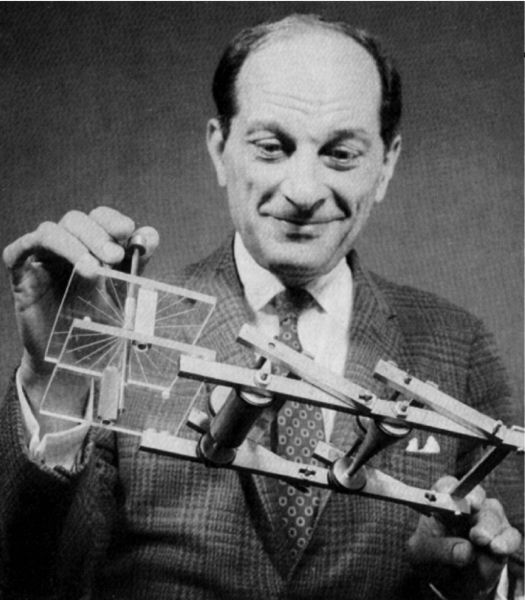
\includegraphics[width=0.25\textwidth]{img/ulam-fermiac.jpg}
\end{center}
{\small
\item Ulam holding the Fermiac, Enrico Fermi's physical Monte Carlo simulator
for random neutron diffusion}
\end{itemize}



\mypart{Appendix I}{Bayesian Data Analysis}

\sld{Bayesian Data Analysis}
\begin{itemize}
\item ``By {Bayesian data analysis}, we mean {practical methods}
for making {inferences} from {data} using {probability models}
for quantities we {observe} and about which we {wish to learn}.''
%
\item ``The essential characteristic of Bayesian methods is
their \myemph{explict use of probability for quantifying uncertainty}
in inferences based on statistical analysis.''
\end{itemize}
%
\vfill\hfill{\footnotesize Gelman et al., {\slshape Bayesian Data Analysis},
  3rd edition, 2013}


\sld{Bayesian Mechanics}
%
\begin{enumerate}
\item Set up full probability model 
\vspace*{-4pt}
\begin{itemize}
\item for all observable \& unobservable quantities
\item consistent w. problem knowledge \& data collection
\end{itemize}
%
\item Condition on observed data
\vspace*{-4pt}
\begin{itemize}
\item caclulate posterior probability of unobserved quantities
  conditional on observed quantities
\end{itemize}
%
\item Evaluate 
\vspace*{-4pt}
\begin{itemize}
\item model fit 
\item implications of posterior
\end{itemize}
\end{enumerate}

\vfill\hfill {\footnotesize {\slshape Ibid.}}

\sld{Basic Quantities}
%
\begin{itemize}
\item Basic Quantities
\vspace*{-4pt}
\begin{itemize}
\item $y$: \ observed data
\item $\tilde{y}$: \ unknown, potentially observable quantities
\item $\theta$: \ parameters (and other unobserved quantities)
\item $x$: \ constants, predictors for conditional models
\end{itemize}
\item Random models for things that could've been otherwise
\begin{itemize}
\item Everyone: Model data $y$ as random
\item Bayesians:  Model parameters $\theta$ as random
\end{itemize}
\end{itemize}


\sld{Distribution Naming Conventions}

\begin{itemize}
\item \myemph{Joint}: \ $p(y,\theta)$
\item \myemph{Sampling / Likelihood}: \ $p(y|\theta)$
\item \myemph{Prior}: \ $p(\theta)$
\item \myemph{Posterior}: \ $p(\theta|y)$
\item \myemph{Data Marginal}: \ $p(y)$
\item \myemph{Posterior Predictive}: \ $p(\tilde{y}|y)$
\end{itemize}

\noindent
\spc
{\footnotesize $y$ modeled data, \, $\theta$ parameters, \, $\tilde{y}$ predictions,}
\\[4pt]
\spc
{\footnotesize implicit: $x, \tilde{x}$ unmodeled data (for $y$, $\tilde{y}$), \ size constants}

\sld{Bayes's Rule for the Posterior}
%
\begin{itemize}
\item Suppose the data $y$ is fixed (i.e., observed).  Then
%
\vspace*{2pt}
\begin{eqnarray*}
p(\theta|y) 
 \hspace*{8pt} = \hspace*{8pt} \frac{p(y,\theta)}{p(y)}
& = & \frac{p(y|\theta) \, p(\theta)}{p(y)}
\\[6pt]
& = & \frac{p(y|\theta) \, p(\theta)}{\int p(y,\theta) \ d\theta}
\\[6pt]
& = & \frac{p(y|\theta) \, p(\theta)}{\int p(y|\theta) \, p(\theta) \ d\theta}
\\[6pt]
& \propto & p(y|\theta) \, p(\theta) \ \ = \ \ p(y,\theta)
\end{eqnarray*}
\item Posterior proportional to likelihood times prior (i.e., joint)
\end{itemize}


\sld{Monte Carlo Methods}
\begin{itemize}
\item For integrals that are impossible to solve analytically
\item But for which sampling and evaluation is tractable
\item Compute plug-in estimates of statistics based on
randomly generated variates (e.g., means, variances,
quantiles/intervals, comparisons)
\item Accuracy with $M$ (independent) samples proportional to
\[
\frac{1}{\sqrt{M}}
\]
e.g., 100 times more samples per decimal place!
\end{itemize}
\vfill\hfill
{\small (Metropolis and Ulam 1949)}


\sld{Monte Carlo Example}
\begin{itemize}
\item Posterior expectation of $\theta$:
\[
\mathbb{E}[\theta|y] = \int \theta \ p(\theta|y) \ d\theta.
\]
\item Bayesian estimate minimizing expected square error: 
\[
\hat{\theta} 
= \arg\min_{\theta'}
\mathbb{E}[(\theta - \theta')^2|y]
= \mathbb{E}[\theta|y] 
\]
\item Generate samples $\theta^{(1)}, \theta^{(2)}, \ldots,
 \theta^{(M)}$ drawn from $p(\theta|y)$
\item Monte Carlo Estimator plugs in average for expectation:
\[
\mathbb{E}[\theta|y] \approx \frac{1}{M} \sum_{m=1}^M \theta^{(m)}
\]
\end{itemize}

\sld{Monte Carlo Example II}
\begin{itemize}
\item Bayesian alternative to frequentist hypothesis testing
\item Use probability to summarize results
\item Bayesian comparison: probability $\theta_1 > \theta_2$ given
  data $y$?
\begin{eqnarray*}
\mbox{Pr}[\theta_1 > \theta_2|y] 
& = & 
\int \int 
\mathbb{I}(\theta_1 > \theta_2) \ p(\theta_1|y) \ p(\theta_2|y)  
\ d\theta_1 \ d\theta_2
\\
& \approx & 
\frac{1}{M} \sum_{m=1}^M \mathbb{I}(\theta_1^{(m)} > \theta_2^{(m)})
\end{eqnarray*}
%
\item (Bayesian hierarchical model ``adjusts'' for multiple comparisons)
\end{itemize}

\sld{Markov Chain Monte Carlo}
\begin{itemize}
\item When sampling independently from $p(\theta|y)$ impossible
\item $\theta^{(m)}$ drawn via a Markov chain $p(\theta^{(m)}|y,\theta^{(m-1)})$
\item Require MCMC marginal $p(\theta^{(m)}|y)$ equal to true
  posterior marginal
\item Leads to auto-correlation in samples
  $\theta^{(1)},\ldots, \theta^{(m)}$
\item Effective sample size $N_{\mbox{\tiny eff}}$ divides out
  autocorrelation (must be estimated)
\item Estimation accuracy proportional to $1 / \sqrt{N_{\mbox{\tiny eff}}}$
\end{itemize}

\sld{Gibbs Sampling}
\begin{itemize}
\item Samples a parameter given data and other parameters
\item Requires conditional posterior $p(\theta_n|y,\theta_{-n})$
\item Conditional posterior easy in directed graphical model
\item Requires general unidimensional sampler for non-conjugacy

\begin{itemize}
\item JAGS uses slice sampler
\item BUGS uses adaptive rejection sampler
\end{itemize}
\item Conditional sampling and general unidimensional sampler 
can both lead to slow convergence and mixing
\end{itemize}
\vfill\hfill
{\small (Geman and Geman 1984)}

\sld{Metropolis-Hastings Sampling}
\begin{itemize}
\item Proposes new point by changing all parameters randomly
\item Computes accept probability of new point based
on ratio of new to old log probability (and proposal density)
\item Only requires evaluation of $p(\theta|y)$
\item Requires good proposal mechanism to be effective
\item Acceptance requires small changes in log probability
\item But small step sizes lead to random walks and slow convergence
  and mixing
\end{itemize}
\vfill\hfill
{\small (Metropolis et al. 1953; Hastings 1970)}


\end{document}


